\begin{figure}[H]
    \centering
    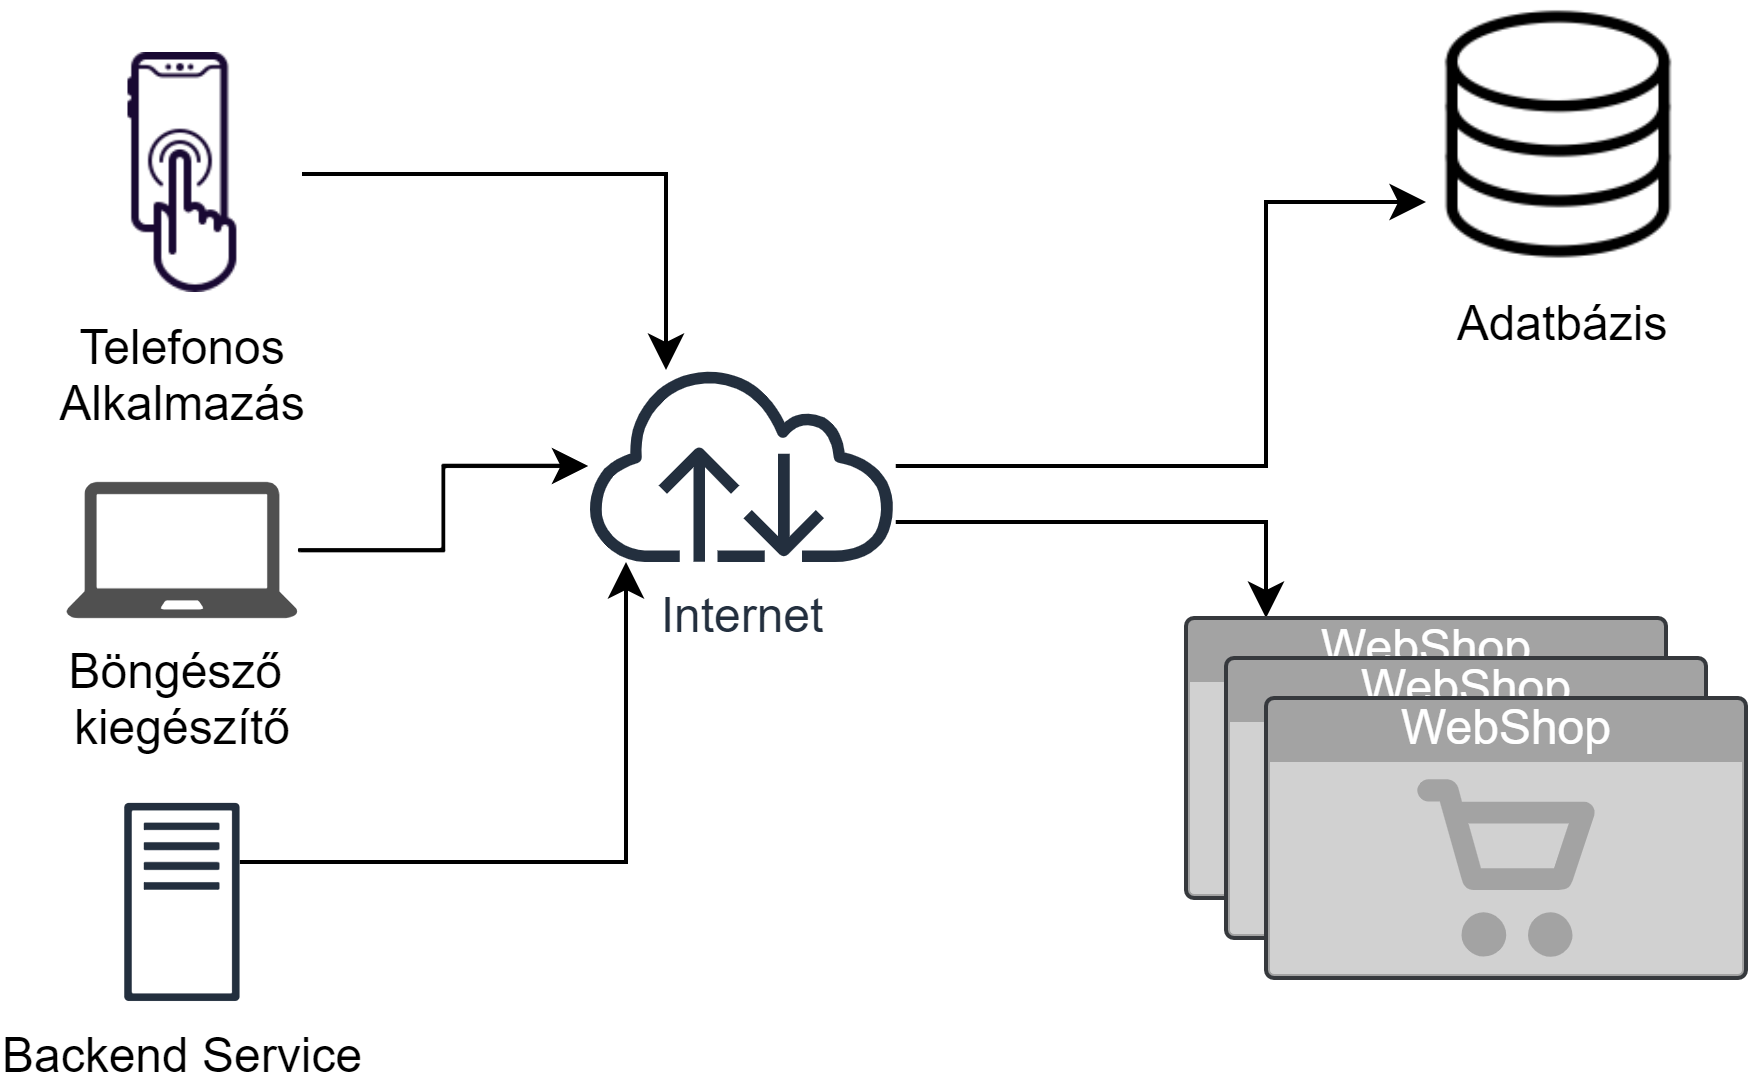
\includegraphics[scale=1.2]{figures/images/architecture_horizontal_HU.png}
    \caption{A rendszer architektúrája}
    \label{fig:architecture}
\end{figure}

A rendszer alapvető részét képezi az adatbázis, amely az adatok tárolását, illetve az azokat elérő API-t szolgáltatja. Ehhez az adatbázishoz két alapvető típusú készülék csatlakozik. A felhasználó oldali, amely lehet akár böngésző kiegészítő vagy telefonos alkalmazás, illetve a szerver vagy logika oldali, amely az adatok feldolgozását biztosító logikát és erőforrást tartalmazza, utóbbi a \ref{fig:architecture} ábrán Backend Service-ként van jelölve. 

A böngésző kiegészítő szükséges, mivel sokkal gyorsabban el lehet érni a megtekinteni kívánt adatokat, valamint sokkal egyszerűbbé teszi a termékek hozzáadását azzal, hogy a követni kívánt termék oldalát egyáltalán nem kell elhagyni. Továbbá fontos, hogy az alkalmazás tudja azt, hogy a felhasználó épp milyen oldalon tartózkodik, ahhoz, hogy a megfelelő URL-t kapja meg, mindezt a kiegészítő könnyen és megbízhatóan el tudja végezni.

Mivel azonban nem mindig vagyunk laptop vagy asztali gép közelben, ezért lehetőséget nyújtunk arra, hogy telefonos applikáció segítségével is el lehessen érni a követett termékeket, valamint minden ehhez tartozó műveletet, akárcsak az előbb említett kiegészítő esetén. Egy termék hozzáadása ezúttal az operációs rendszer megosztási menüjén keresztül történik, ami által az alkalmazás megkapja a követni kívánt termék elérhetőségét.

Ahhoz, hogy az eszközök kommunikálni tudjanak egymással, egyértelmű, hogy szükség van valamiféle összeköttetésre, amely a mi esetünkben az internet lesz. Ez a funkció létfontosságú, mivel minden adatot fel, illetve le kell tölteni az adatbázisból, függetlenül az eszközök tartózkodási helyétől, ugyanakkor a szolgáltatást biztosító rendszer is ezen keresztül éri el a termékek weboldalát.

Az architektúra fontos részét képezik a webshop-ok is, mivel ezeket úgy a termék hozzáadásakor, mint azoknak periodikus ellenőrzésekor el kell érni, az adatok begyűjtése érdekében. A támogatott webshop-ok főként népszerűségüket tekintve lettek kiválasztva, mint például az Emag, viszont ezen kívül két más webáruház is támogatott, ezek a Flanco és QuickMobile. Mivel minden weboldal másképp épül fel, mindegyik oldal struktúrájából másképp kell kinyerni az adatokat, ezért ezt a folyamatot személyre szabottan kell végezni. Ugyanakkor változhatnak is idővel ezek a struktúrák, ezeket figyelni kell. 

\section{A modulok megvalósítása}

\subsection{Chrome Extension}

A böngésző kiegészítő vagy angolul browser extension, egy a böngésző környezetén belül futó alkalmazás, ami olyan funkciókat hivatott hozzáadni a felhasználói felülethez, melyek megkönnyítik vagy jobbá teszik a felhasználóii élményt. Előnye, hogy alkalmazások ezrei állnak a felhasználok rendelkezésére, melyeket par kattintással telepíthetnek is. Ezek már szinte minden böngészőn megtalálhatók valamilyen formában, a legnépszerűbbek esetében, mint például, Google Chrome, Firefox ez a funkció régóta jelen van.

Ezen kiegészítők működése valószínűleg sokak számára ismert, amolyan lenyíló ablakként jelennek meg a böngészőben, anélkül, hogy hatással lennének az éppen megjelenített tartalomra. Ennek tudatában, ez a megközelítés tűnt a legmegfelelőbbnek a dolgozatban tárgyalt szoftver felhasználói felületének elkészítése során. Mivel ezek a funkciók csak asztali gépeken érhetőek el, ezért szükséges volt egy telefonos interface kifejlesztése is, mely a későbbiekben kerül bemutatásra.

A kiegészítő megvalósítása során, JavaScript, HTML, CSS programozási nyelvek voltak felhasználva. Mivel korábban nem volt tapasztalatom böngészőhöz való kiegészítők fejlesztésében, ezért az implementálási folyamat információ gyűjtéssel kezdődött. Utánanéztem hogyan is zajlik egy ilyen kiegészítő fejlesztése, mik a követendő lepések illetve fázisok.

Első lépésben szükséges egy manifest.json file létrehozása, mely a kiegészítő alapvető információit tartalmazza, mint például verziószám, név, rövid leírás, felhasznált függőségek, engedélyezett műveletek stb... . Ezek után, a fejlesztés hasonló egy hagyományos weboldal elkészítéséhez. 

A fejlesztés során több könyvtár került felhasználásra, különböző funkciók ellátására, ezek a Bootstrap, sweetalert2, firebase, amcharts. A bootstrap egy ingyenes, nyílt forráskádul CSS framework, mely segítségével interaktívabbá, szebbé tehetjük a weboldalunkat, előre definiált mintákat biztosit nekünk, gombok, navigáció vagy más komponensek esetében. A sweetalert2 egy úgynevezett riasztásokért felelős könyvtár, olyan esetekben került használatra, amikor egy felugró ablak segítségével szeretnénk megerősítést kérni a felhasználótól egy bizonyos művelet elvégzésére, mint például termékek törlése vagy kijelentkezés során, viszont egyéb, információ közlési célokra is felhasználva lett, mint például egy művelet sikeres elvégzésének visszajelzése. A firebase könyvtárakat bejelentkezési, valamint adatbázis kezelő funkciók miatt volt szükséges használni. Az árak időbeli változását ábrázoló diagramok eseteben több könyvtárat is kipróbáltam, viszont a végső választás az amcharts nevűre eset, mivel ez volt a leg megfelelőbb az adott esetben.

Amikor a felhasználó először használja a kiegészítőt, egy login oldal jelenik meg számára, melyen be tud jelentkezni, valamint regisztrálni tud \ref{fig:ext_login_reg}.

\begin{figure}[H]
    \centering
    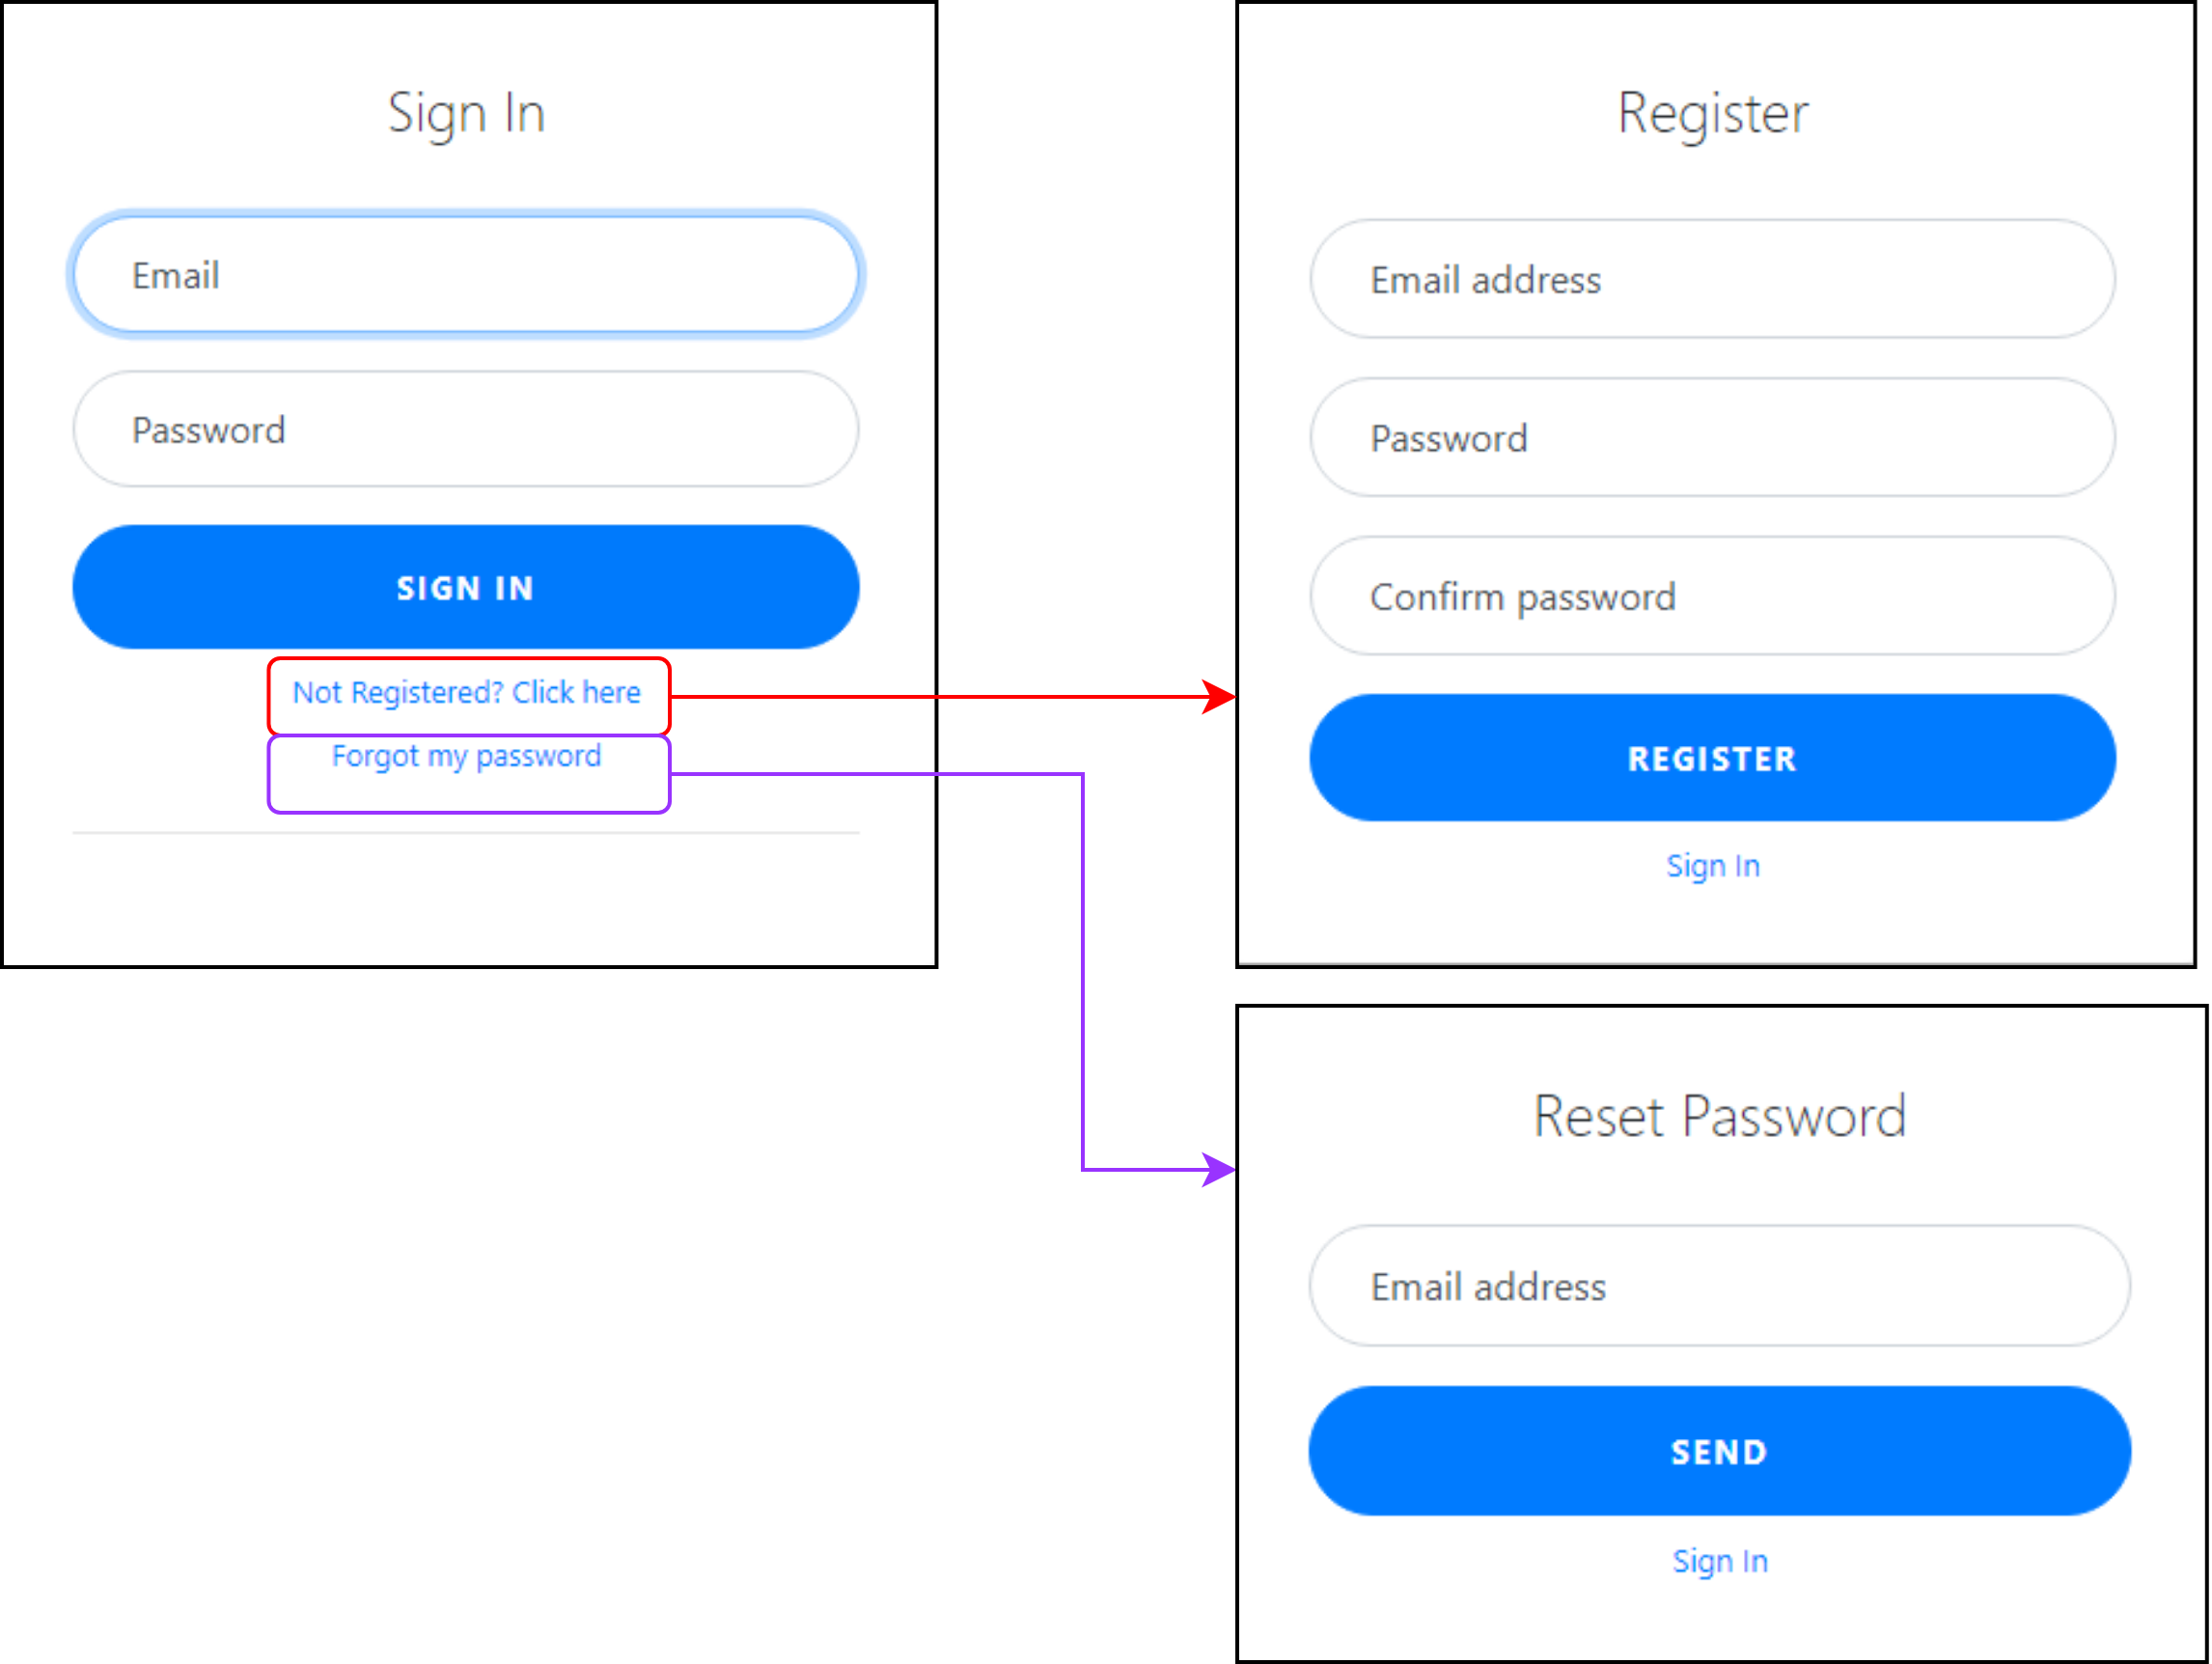
\includegraphics[scale=1]{figures/images/login-reg-ext.png}
    \caption{Kiegeszito bejelentkezési/regisztrálási felülete}
    \label{fig:ext_login_reg}
\end{figure}